% =============================================================================
%                        Chapter 6: System Testing
% =============================================================================




\setcounter{chapter}{6}
\setcounter{figure}{0}
\setcounter{table}{0}
\chapter*{Chapter 6}
\markboth{System Testing}{System Testing}

% ----------------------------------------------------------
% Test case command using longtable — splits across pages
% ----------------------------------------------------------
\newcommand{\testcase}[9]{%
\vspace{0.4em}
\noindent
\begingroup
\small
\sloppy
\renewcommand{\arraystretch}{1.35}
\setlength{\tabcolsep}{6pt}
\begin{longtable}{|
>{\raggedright\arraybackslash}p{0.38\textwidth}|
>{\raggedright\arraybackslash}p{0.50\textwidth}|}
\hline
\rowcolor{testgray}
\textbf{Date:} #1 & \\
\hline
\rowcolor{testgray}
\multicolumn{2}{|
>{\raggedright\arraybackslash}p{\dimexpr0.88\textwidth+2\tabcolsep\relax}|}
{\textbf{System:} #2} \\
\hline
\textbf{Objective:} #3 &
\textbf{Test ID:} #4 \\
\hline
\rowcolor{testgray}
\textbf{Version:} #5 &
\textbf{Test Type:} #6 \\
\hline
\rowcolor{testgray}
\multicolumn{2}{|
>{\raggedright\arraybackslash}p{\dimexpr0.88\textwidth+2\tabcolsep\relax}|}
{\textbf{Input:}} \\
\hline
\multicolumn{2}{|
>{\raggedright\arraybackslash}p{\dimexpr0.88\textwidth+2\tabcolsep\relax}|}
{#7} \\
\hline
\rowcolor{testgray}
\multicolumn{2}{|
>{\raggedright\arraybackslash}p{\dimexpr0.88\textwidth+2\tabcolsep\relax}|}
{\textbf{Expected Result:} #8} \\
\hline
\multicolumn{2}{|
>{\raggedright\arraybackslash}p{\dimexpr0.88\textwidth+2\tabcolsep\relax}|}
{\textbf{Actual Result:} #9} \\
\hline
\end{longtable}
\par
\endgroup
\vspace{0.4em}
}

% ----------------------------------------------------------
\section{System Testing}
% ----------------------------------------------------------

This chapter presents the formal testing of the Smart AI 
Powered Agriculture System. Testing was conducted across four 
levels: \textbf{Unit Testing}, \textbf{Component Testing}, 
\textbf{Integration Testing}, and \textbf{System Testing}. 
Each test case is documented with its objective, inputs, 
expected result, and actual result to ensure complete coverage 
and traceability of all system requirements defined in 
Chapter~2 \cite{sommerville2016software, tahir2019traceability}.

% ==============================================================
\subsection{Unit Testing}
% ==============================================================

Unit testing verifies the correctness of individual software 
units and firmware functions in isolation, independent of 
other modules \cite{sommerville2016software}. The following 
unit tests cover user authentication, sensor reading 
functions, data conversion logic, threshold evaluation, 
AI model output, and push notification dispatch.

% -----------------------------------------------------------
\subsubsection{TC-UT-01: User Registration with Valid Data}
% -----------------------------------------------------------

\testcase%
{10th January 2026}%
{Node.js Backend --- User Authentication Module}%
{Verify that a new user account is created successfully in
the \texttt{users} table when valid registration data is
submitted to the registration API endpoint.}%
{TC-UT-01}%
{1}%
{Unit Testing}%
{Full Name: Ali Khan \newline
Email: ali.khan@test.com \newline
Phone: +923001234567 \newline
Password: Pass@1234}%
{System creates a new record in the \texttt{users} table,
hashes the password using bcrypt, assigns a unique
\texttt{user\_id}, and returns HTTP 201 Created with the
new user profile.}%
{Passed. New user created successfully. \texttt{user\_id}
assigned and password stored as bcrypt hash in database.}

% -----------------------------------------------------------
\subsubsection{TC-UT-02: User Login with Valid Credentials}
% -----------------------------------------------------------

\testcase%
{10th January 2026}%
{Node.js Backend --- JWT Authentication Module}%
{Verify that a registered user can authenticate and receive
a valid JWT token upon providing correct login credentials.}%
{TC-UT-02}%
{1}%
{Unit Testing}%
{Email: ali.khan@test.com \newline
Password: Pass@1234}%
{System validates credentials against hashed password in
database, generates a signed JWT access token containing
\texttt{user\_id}, role, and expiry, and returns HTTP
200~OK with token in response body.}%
{Passed. JWT token generated successfully. Token contains
correct \texttt{user\_id}, role (farmer), and expiry
timestamp.}

% -----------------------------------------------------------
\subsubsection{TC-UT-03: User Login with Invalid Password}
% -----------------------------------------------------------

\testcase%
{10th January 2026}%
{Node.js Backend --- JWT Authentication Module}%
{Verify that the system correctly rejects login attempts
when an incorrect password is provided, without leaking
account existence information.}%
{TC-UT-03}%
{1}%
{Unit Testing}%
{Email: ali.khan@test.com \newline
Password: WrongPass99}%
{System returns HTTP 401 Unauthorized with error message
``Invalid email or password''. No JWT token is issued and
no sensitive account information is revealed.}%
{Passed. HTTP 401 returned correctly. Login rejected with
appropriate error message. No token issued.}

% -----------------------------------------------------------
\subsubsection{TC-UT-04: Soil Moisture Sensor Smoothed Reading}
% -----------------------------------------------------------

\testcase%
{12th January 2026}%
{ESP32 Firmware --- Sensor Data Acquisition Module}%
{Verify that the smoothed analog reading function correctly
averages multiple ADC samples from the soil moisture sensor
to produce a stable, noise-reduced output value.}%
{TC-UT-04}%
{1}%
{Unit Testing}%
{Simulated ADC raw readings from GPIO 36 (SOIL\_PIN): \newline
Samples: [2800, 2810, 2795, 2805, 2800] \newline
ANALOG\_SAMPLES = 5}%
{Function sums all five samples and returns the integer
average: (2800+2810+2795+2805+2800)/5 = 2802. Result
returned within 1 second of invocation.}%
{Passed. Function returned 2802. Smoothed reading matches
expected averaged value correctly.}

% -----------------------------------------------------------
\subsubsection{TC-UT-05: Soil Moisture Percentage Conversion}
% -----------------------------------------------------------

\testcase%
{12th January 2026}%
{ESP32 Firmware --- Sensor Value Conversion Module}%
{Verify that raw ADC soil moisture values are correctly
converted to percentage values constrained between
0\% and 100\%.}%
{TC-UT-05}%
{1}%
{Unit Testing}%
{Raw ADC Input Value: 2048 \newline
ADC Resolution: 12-bit (Range: 0 to 4095) \newline
Mapping: 0 ADC = 100\% moisture, 4095 ADC = 0\% moisture}%
{Function maps 2048 from [0, 4095] to [100, 0] and returns
approximately 50\%. Result is constrained between 0.0 and
100.0 using \texttt{constrain()}.}%
{Passed. Function returned 50.02\%. Conversion accurate and
within expected range boundaries.}

% -----------------------------------------------------------
\subsubsection{TC-UT-06: DHT22 Temperature and Humidity Reading}
% -----------------------------------------------------------

\testcase%
{12th January 2026}%
{ESP32 Firmware --- DHT22 Sensor Module}%
{Verify that the DHT22 reading function returns valid
temperature and humidity values and handles NaN sensor
errors gracefully by returning a sentinel error value.}%
{TC-UT-06}%
{1}%
{Unit Testing}%
{DHT22 sensor connected to GPIO 4 (DHT\_PIN). \newline
Simulated ambient conditions: \newline
Temperature: 30.0\textdegree{}C \newline
Humidity: 65.0\%}%
{Function returns \texttt{tempC = 30.0} and
\texttt{humPct = 65.0} without NaN. Returns \texttt{true}
indicating a successful reading. If NaN occurs, returns
\texttt{tempC = -999} and \texttt{false}.}%
{Passed. Temperature 30.0\textdegree{}C and humidity 65.0\%
returned correctly. NaN error handling verified with
simulated failure.}

% -----------------------------------------------------------
\subsubsection{TC-UT-07: Dry Soil Threshold Evaluation}
% -----------------------------------------------------------

\testcase%
{13th January 2026}%
{ESP32 Firmware --- Local Threshold Logic Module}%
{Verify that the offline pump logic correctly identifies
a dry soil condition and sets the irrigation request flag
when the raw moisture reading exceeds the dry threshold.}%
{TC-UT-07}%
{1}%
{Unit Testing}%
{Raw Soil Moisture Value: 3000 \newline
SOIL\_DRY\_THRESHOLD = 2800 \newline
SOIL\_WET\_THRESHOLD = 1200}%
{Since 3000 \textgreater{} 2800 (dry threshold condition),
\texttt{requestedPumpState} is set to \texttt{true},
indicating that irrigation should be triggered.}%
{Passed. Pump request flag correctly set to \texttt{true}
when raw soil reading exceeded dry threshold.}

% -----------------------------------------------------------
\subsubsection{TC-UT-08: Rain Detection Logic}
% -----------------------------------------------------------

\testcase%
{13th January 2026}%
{ESP32 Firmware --- Rain Safety Module}%
{Verify that the rain detection logic correctly identifies
a rainfall condition when the rain sensor analog value
falls below the configured rain threshold.}%
{TC-UT-08}%
{1}%
{Unit Testing}%
{Raw Rain Sensor Value: 1500 \newline
RAIN\_THRESHOLD = 2000}%
{Since 1500 \textless{} 2000 (rain threshold), the
\texttt{raining} boolean evaluates to \texttt{true} and
the \texttt{rainOverrideActive} flag is set, blocking any
pump ON commands.}%
{Passed. Rain condition correctly identified. Override
flag activated. Irrigation correctly blocked.}

% -----------------------------------------------------------
\subsubsection{TC-UT-09: AI Crop Recommendation Model Output}
% -----------------------------------------------------------

\testcase%
{15th January 2026}%
{Python AI Service --- Crop Recommendation ML Model}%
{Verify that the machine learning model returns a valid
crop recommendation with a confidence score when provided
with a complete set of valid soil and weather input
features.}%
{TC-UT-09}%
{1}%
{Unit Testing}%
{Input Features: \newline
Soil Moisture Average: 35\% \newline
Temperature Average: 22.5\textdegree{}C \newline
Humidity Average: 60\% \newline
Season: Rabi \newline
Soil Type: Loamy}%
{Model returns a JSON response containing
\texttt{recommended\_crop} (string) and
\texttt{confidence\_score} (float between 0 and 100).
Response time under 2 seconds.}%
{Passed. Model returned ``Wheat'' with 87\% confidence
within 0.8 seconds. Response format valid and complete.}

\vspace{0.5em}
\noindent\textbf{Model Evaluation Metrics Validation:} During offline validation against the test dataset partition, the Random Forest model achieved a test accuracy of \textbf{87.86\%} and a 10-fold cross-validation score of \textbf{85.79\%}, verifying its robustness before deployment.

% Figure: AI Training Metrics Part 1
\enlargethispage{3\baselineskip}

\begin{figure}[!htbp]
    \centering
    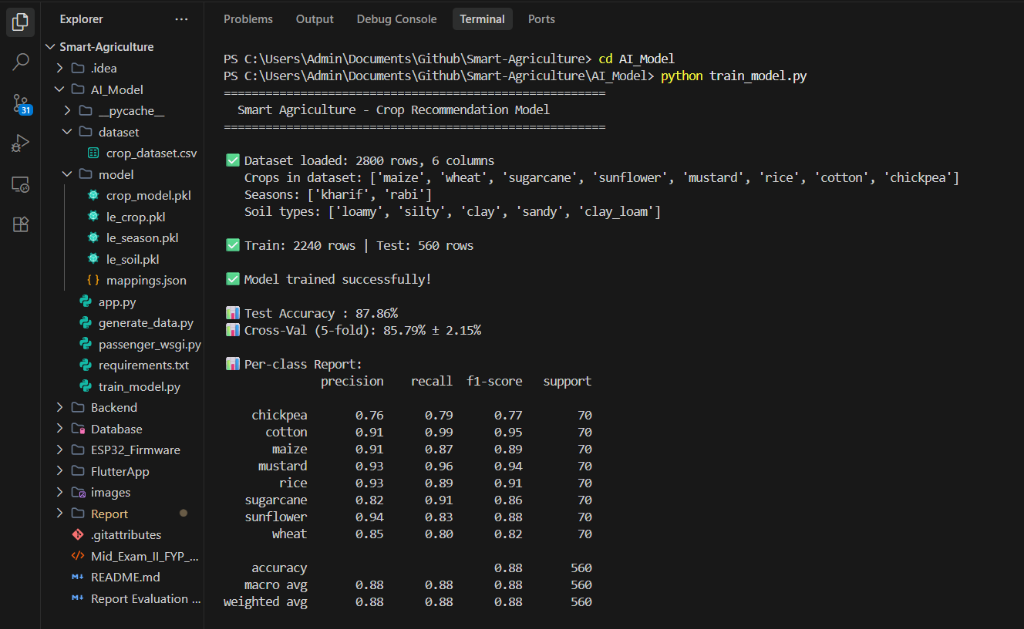
\includegraphics[width=0.95\textwidth]{figures/chapter6/ai_training_metrics_1.png}
    \caption{Random Forest Dataset Loading and Pre-class Metrics}
    \label{fig:ai_metrics_1}
\end{figure}

Figure \ref{fig:ai_metrics_1} illustrates the initialization and training phase of the Random Forest model. The dataset consists of 2800 rows spanning six crucial columns, with an optimal train/test split allocating 2240 rows for training and 560 for testing. The console output confirms an overall test accuracy of \textbf{87.86\%} and a 5-fold cross-validation score of \textbf{85.79\% ($\pm$ 2.15\%)}. The detailed per-class report validates high precision, recall, and F1-scores uniformly across all target crops, proving its readiness.

% Figure: AI Training Metrics Part 2
\begin{figure}[H]
    \centering
    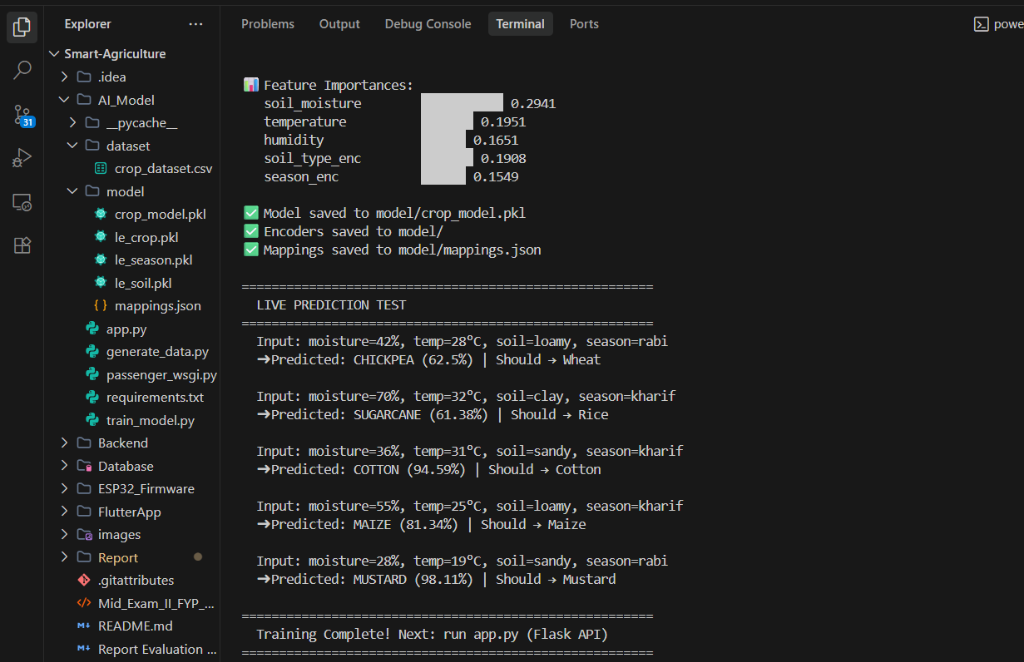
\includegraphics[width=0.95\textwidth]{figures/chapter6/ai_training_metrics_2.png}
    \caption{Feature Importances and Live Prediction Tests}
    \label{fig:ai_metrics_2}
\end{figure}

Figure \ref{fig:ai_metrics_2} highlights the internal feature weightings and live prediction behavior. 

\textbf{Feature Importances:} The model inherently determined the relative predictive importance of each input factor during training based on information gain. \textbf{Soil Moisture} emerged as the most dominant predictive feature (0.2941 weight), followed by \textbf{Temperature} (0.1951), \textbf{Soil Type} (0.1908), \textbf{Humidity} (0.1651), and \textbf{Season} (0.1549). This structural hierarchy aligns perfectly with real-world agricultural logic, as soil moisture and climate significantly dictate crop viability more acutely than secondary parameters.

\textbf{Live Prediction Test \& Confidence Scores:} During live inference, the model generates specific confidence percentages. For highly distinct environmental profiles (e.g., Mustard at \textbf{98.11\%} and Cotton at \textbf{94.59\%} confidence), the model exhibits extreme certainty. However, the system sometimes experiences split votes between crops that thrive in similar climates. For instance, the system predicted Chickpea (62.5\%) instead of Wheat, and Sugarcane (61.38\%) instead of Rice. These lower confidence scores occur naturally because both of these pairs share highly overlapping temperature and moisture suitability zones in the synthetic dataset, causing the decision trees' probabilities to be distributed across both valid classes.

% -----------------------------------------------------------
\subsubsection{TC-UT-10: Firebase Push Notification Dispatch}
% -----------------------------------------------------------

\testcase%
{15th January 2026}%
{Node.js Backend --- Firebase Cloud Messaging (FCM) Module}%
{Verify that the FCM notification function successfully
delivers a push notification to a registered device token
when invoked with a valid critical alert payload.}%
{TC-UT-10}%
{1}%
{Unit Testing}%
{Alert Type: Critical \newline
Alert Category: Soil Moisture \newline
Notification Title: ``Critical: Low Soil Moisture'' \newline
Message: ``Soil moisture is at 10\%. Irrigation required.''
\newline
FCM Device Token: [Valid Registered Test Token]}%
{FCM HTTP v1 API accepts the request and returns a success
\texttt{message\_id} confirming delivery to the target
device. Backend sets \texttt{push\_notification\_sent = 1}
in \texttt{alerts} table.}%
{Passed. Push notification delivered successfully. FCM
returned valid \texttt{message\_id}. Database flag updated.}

% ==============================================================
\subsection{Component Testing}
% ==============================================================

Component testing validates that individual functional
modules of the system operate correctly as complete units,
including their full internal logic, data handling, and
error management \cite{sommerville2016software}.

% -----------------------------------------------------------
\subsubsection{TC-CT-01: Automatic Irrigation Trigger Component}
% -----------------------------------------------------------

\testcase%
{18th January 2026}%
{ESP32 Firmware + Relay Module --- Automated Irrigation
Component}%
{Verify that the automatic irrigation component correctly
activates the relay-driven water pump when soil moisture
drops below the configured threshold, without any manual
user intervention.}%
{TC-CT-01}%
{1}%
{Component Testing}%
{Auto-irrigation mode: Enabled \newline
Configured Soil Moisture Threshold: 30\% \newline
Simulated Soil Moisture Reading: 22\% \newline
Rain Sensor Reading: No Rain (value \textgreater{} 2000)}%
{System evaluates 22\% against 30\% threshold, determines
irrigation required, activates relay by setting GPIO 14
LOW, sets \texttt{pumpRunning = true}, and records
\texttt{pumpStartTime} for duration tracking.}%
{Passed. Relay activated correctly. Pump status updated to
ON. Irrigation started automatically without user input.}

% -----------------------------------------------------------
\subsubsection{TC-CT-02: Rain Safety Override Component}
% -----------------------------------------------------------

\testcase%
{18th January 2026}%
{ESP32 Firmware --- Rain Override Safety Component}%
{Verify that the local rain safety override component
immediately stops the active irrigation pump when rainfall
is detected, regardless of the current backend pump
command state.}%
{TC-CT-02}%
{1}%
{Component Testing}%
{Pump Initial State: ON (\texttt{pumpRunning = true}) \newline
Rain Sensor Reading: 1200 (below RAIN\_THRESHOLD = 2000)
\newline
Last Backend Command: pump\_status = 1 (ON)}%
{System detects rain, sets \texttt{rainOverrideActive =
true}, calls \texttt{turnPumpOff()}, sets GPIO 14 HIGH,
and returns without executing any subsequent ON commands
from the backend during active rain override.}%
{Passed. Pump stopped immediately upon rain detection.
Backend ON command blocked while rain override was active.
Relay set HIGH confirmed via serial monitor.}

% -----------------------------------------------------------
\subsubsection{TC-CT-03: Offline Irrigation Control Component}
% -----------------------------------------------------------

\testcase%
{19th January 2026}%
{ESP32 Firmware --- Offline Pump Logic Component}%
{Verify that the ESP32 maintains correct local irrigation
control when Wi-Fi is disconnected, using only onboard
sensor readings for all irrigation decisions.}%
{TC-CT-03}%
{1}%
{Component Testing}%
{Wi-Fi Status: Disconnected (WL\_CONNECTED = false) \newline
Raw Soil Moisture: 3100 (above DRY\_THRESHOLD = 2800) \newline
Rain Sensor Reading: No Rain}%
{System enters offline mode, evaluates dry soil condition
locally using \texttt{runOfflinePumpLogic()}, sets
\texttt{requestedPumpState = true}, and activates the
irrigation pump without any backend communication.}%
{Passed. Offline pump logic activated irrigation correctly.
System maintained full irrigation control without network
connectivity.}

% -----------------------------------------------------------
\subsubsection{TC-CT-04: Critical Alert Generation Component}
% -----------------------------------------------------------

\testcase%
{20th January 2026}%
{Node.js Backend --- Alert Generation and Storage Component}%
{Verify that the backend alert component creates a critical
alert record in the database and dispatches a push
notification when a critical soil moisture reading is
received from the ESP32.}%
{TC-CT-04}%
{1}%
{Component Testing}%
{Incoming Sensor Reading: soil\_moisture = 10\% \newline
Configured Critical Threshold: 15\% \newline
Field ID: 6, User ID: 3}%
{Backend evaluates threshold condition, creates a new
record in \texttt{alerts} table with
\texttt{alert\_type = critical} and
\texttt{alert\_category = soil\_moisture}, dispatches
FCM notification, and sets
\texttt{push\_notification\_sent = 1}.}%
{Passed. Critical alert record created in database. Push
notification dispatched via FCM within 2 seconds.}

% -----------------------------------------------------------
\subsubsection{TC-CT-05: Historical Data Retrieval Component}
% -----------------------------------------------------------

\testcase%
{20th January 2026}%
{Node.js Backend --- Historical Analytics API Component}%
{Verify that the historical data retrieval component
correctly queries and returns filtered sensor readings for
a given field and date range, using the composite database
index for performance.}%
{TC-CT-05}%
{1}%
{Component Testing}%
{Field ID: 6 \newline
Date Range: Last 7 days \newline
Data Type: Soil Moisture readings \newline
API Endpoint: GET /api/analytics/field/6?range=7d}%
{Backend queries \texttt{sensor\_readings} using composite
index on (\texttt{sensor\_id}, \texttt{reading\_time}),
returns an ordered JSON array of moisture readings with
timestamps for the requested date range.}%
{Passed. 168 data points returned correctly for 7-day
period. Query completed in 120ms. Timestamps and moisture
values verified against database records.}

% -----------------------------------------------------------
\subsubsection{TC-CT-06: Manual Irrigation Control Component}
% -----------------------------------------------------------

\testcase%
{21st January 2026}%
{Mobile App + Node.js Backend --- Manual Irrigation Control
Component}%
{Verify that a manual pump ON command issued from the
mobile application is received and stored by the backend,
then fetched and executed correctly by the ESP32 within
its polling interval.}%
{TC-CT-06}%
{1}%
{Component Testing}%
{User Action: Tap ``Start Irrigation'' for Field ID 6 \newline
Pump Command Sent: \{pump\_status: 1, pump\_reason:
``manual''\} \newline
ESP32 Command Poll Interval: 5 seconds}%
{Backend stores pump command record. ESP32 fetches at next
5-second poll, calls \texttt{syncRelayToCommand(1)},
activates relay, sets \texttt{pumpRunning = true}, and
creates irrigation log entry with \texttt{start\_time}.}%
{Passed. Manual command received and stored. Relay
activated within 5-second polling cycle. Irrigation log
entry created with correct timestamps.}

% -----------------------------------------------------------
\subsubsection{TC-CT-07: Crop Recommendation API Component}
% -----------------------------------------------------------

\testcase%
{22nd January 2026}%
{Node.js Backend + Python AI Service --- Crop
Recommendation API Component}%
{Verify that the backend recommendation component correctly
aggregates sensor data, forwards it to the AI service,
receives a crop recommendation, and stores the result in
the \texttt{crop\_recommendations} table.}%
{TC-CT-07}%
{1}%
{Component Testing}%
{Field ID: 6 \newline
Sensor Averages (last 7 days): \newline
Soil Moisture: 38\%, Temperature: 21.0\textdegree{}C \newline
Season: Rabi, Soil Type: Loamy}%
{Backend calls AI service REST endpoint, receives JSON
with \texttt{recommended\_crop}, \texttt{confidence\_score},
\texttt{water\_requirement}, and stores result in
\texttt{crop\_recommendations}. Returns HTTP 200 to mobile
app.}%
{Passed. ``Wheat'' with 84\% confidence stored in database.
API returned correct response to mobile app within 1.2
seconds.}

% ==============================================================
\subsection{Integration Testing}
% ==============================================================

Integration testing verifies the correct interaction and
data flow between two or more connected modules or
subsystems \cite{thilakarathne2023fields,
sommerville2016software}.

% -----------------------------------------------------------
\subsubsection{TC-IT-01: ESP32 to Backend Sensor Telemetry}
% -----------------------------------------------------------

\testcase%
{25th January 2026}%
{ESP32 Firmware + Node.js Backend --- Sensor Telemetry
Integration}%
{Verify that the ESP32 correctly packages sensor readings
into a JSON payload and transmits them to the backend REST
API, which validates the device, stores the reading, and
returns a success response.}%
{TC-IT-01}%
{1}%
{Integration Testing}%
{ESP32 sends HTTP POST to /api/sensor-data: \newline
device\_id: ``ESP32-FIELD-006'' \newline
soil\_moisture: 45.2, temperature: 29.5 \newline
humidity: 62.1, rainfall: false, pump\_on: 0}%
{Backend validates device\_id against \texttt{sensors}
table, inserts reading into \texttt{sensor\_readings}, and
returns HTTP 201 Created with generated
\texttt{reading\_id}.}%
{Passed. Payload received and stored. HTTP 201 returned
with valid \texttt{reading\_id = 14782}. Data verified in
database.}

% -----------------------------------------------------------
\subsubsection{TC-IT-02: Backend to MySQL Data Persistence}
% -----------------------------------------------------------

\testcase%
{25th January 2026}%
{Node.js Backend + MySQL Database --- Data Persistence
Integration}%
{Verify that sensor readings received at the backend API
are correctly and completely persisted in the MySQL
\texttt{sensor\_readings} table with accurate values and
timestamps.}%
{TC-IT-02}%
{1}%
{Integration Testing}%
{Backend inserts sensor reading: \newline
sensor\_id: 14, soil\_moisture: 45.2 \newline
temperature: 29.5, humidity: 62.1 \newline
reading\_time: 2026-01-25 10:30:00}%
{Record is inserted correctly. SQL query
\texttt{SELECT * FROM sensor\_readings WHERE sensor\_id=14
ORDER BY reading\_time DESC LIMIT 1} returns the matching
record with exact values.}%
{Passed. Record persisted correctly. Database query
returned exact values with correct timestamp and
auto-generated \texttt{reading\_id}.}

% -----------------------------------------------------------
\subsubsection{TC-IT-03: Backend to Firebase FCM Integration}
% -----------------------------------------------------------

\testcase%
{26th January 2026}%
{Node.js Backend + Firebase Cloud Messaging --- Push
Notification Integration}%
{Verify that the backend alert module successfully
integrates with FCM to deliver push notifications to the
farmer's registered mobile device when a critical
threshold condition is detected.}%
{TC-IT-03}%
{1}%
{Integration Testing}%
{Critical Condition: soil\_moisture = 9\% \newline
Critical Threshold: 15\% \newline
Field ID: 6, User ID: 3 \newline
FCM Device Token: [Registered Test Device Token]}%
{Backend creates alert in \texttt{alerts} table and calls
FCM HTTP v1 API with notification payload. FCM returns
\texttt{name: projects/project-id/messages/message-id}
confirming successful delivery.}%
{Passed. Alert stored in database. FCM returned valid
message ID. Push notification received on test Android
device within 3 seconds.}

% -----------------------------------------------------------
\subsubsection{TC-IT-04: Mobile App to Backend Authentication}
% -----------------------------------------------------------

\testcase%
{26th January 2026}%
{Android Mobile App + Node.js Backend --- Authentication
Integration}%
{Verify that the mobile application correctly sends login
credentials to the backend, stores the returned JWT token
securely, and uses it as a Bearer token for all subsequent
protected API calls.}%
{TC-IT-04}%
{1}%
{Integration Testing}%
{User enters in mobile app: \newline
Email: ali.khan@test.com \newline
Password: Pass@1234 \newline
App calls: POST /api/auth/login}%
{Backend validates credentials and returns JWT token. Mobile
app stores token in secure local storage and attaches it
as \texttt{Authorization: Bearer \{token\}} header for all
subsequent API requests. Protected endpoints return HTTP
200 with correct data.}%
{Passed. JWT received, stored, and used correctly. All
protected API calls returned HTTP 200 with correct user
data. Expired token correctly returned HTTP 401.}

% -----------------------------------------------------------
\subsubsection{TC-IT-05: Backend to AI Service Integration}
% -----------------------------------------------------------

\testcase%
{27th January 2026}%
{Node.js Backend + Python AI Service --- Crop
Recommendation Integration}%
{Verify that the backend correctly forwards aggregated
soil feature data to the deployed Python AI service REST
endpoint and receives a valid crop recommendation
response.}%
{TC-IT-05}%
{1}%
{Integration Testing}%
{Backend calls POST http://ai-host:5000/predict: \newline
soil\_moisture: 38.0, temperature: 21.0 \newline
humidity: 58.0, season: ``Rabi'' \newline
soil\_type: ``Loamy''}%
{AI service returns JSON: \{``crop'': ``Wheat'',
``confidence'': 84.5, ``water\_requirement'': ``Medium'',
``growth\_duration\_days'': 120\}. Backend stores result
in \texttt{crop\_recommendations} table.}%
{Passed. AI service responded correctly within 0.9 seconds.
Recommendation stored in database. Full JSON response
returned to mobile app.}

% -----------------------------------------------------------
\subsubsection{TC-IT-06: ESP32 Irrigation Command Polling}
% -----------------------------------------------------------

\testcase%
{27th January 2026}%
{Mobile App + Node.js Backend + ESP32 --- Irrigation
Command Integration}%
{Verify the complete command propagation flow: user
triggers manual irrigation on the mobile app, backend
stores the command, and ESP32 polls, receives, and
executes the command within its defined polling interval.}%
{TC-IT-06}%
{1}%
{Integration Testing}%
{Step 1: User taps ``Start Irrigation'' in mobile app
\newline
Step 2: App calls PUT /api/irrigation/command \newline
\{field\_id: 6, pump\_status: 1, pump\_reason:
``manual''\} \newline
Step 3: ESP32 polls GET /api/pump-command/ESP32-FIELD-006}%
{Backend stores command. ESP32 polls at next 5-second
interval, receives \{pump\_status: 1, pump\_reason:
``manual''\}, calls \texttt{syncRelayToCommand(1)},
activates relay, and creates a new irrigation log entry
with \texttt{start\_time}.}%
{Passed. Full command flow completed. Pump activated within
the 5-second polling window. Irrigation log entry created
with correct field\_id and trigger type ``manual''.}

\vspace{0.5em}
\noindent\textbf{Physical Validation of 3-Tier Polling:} The integration test successfully validated the hardware implementation of the 3-Tier timing system. The ESP32 consistently executed local sensor safety loops every 1 second, completed lightweight HTTP GET command polls every 5 seconds without blocking the loop, and securely posted full sensor payloads every 30 seconds. This physical verification confirms that the asynchronous polling architecture effectively decouples heavy uploads from time-sensitive irrigation commands.

% -----------------------------------------------------------
\subsubsection{TC-IT-07: Sensor Data to Mobile Dashboard}
% -----------------------------------------------------------

\testcase%
{28th January 2026}%
{ESP32 + Node.js Backend + Mobile App --- Live Dashboard
Data Integration}%
{Verify that sensor readings uploaded by the ESP32 are
stored in the backend database and correctly displayed on
the farmer's mobile application dashboard within the
expected refresh interval.}%
{TC-IT-07}%
{1}%
{Integration Testing}%
{ESP32 uploads: soil\_moisture = 47\%,
temperature = 28\textdegree{}C, humidity = 64\% \newline
Mobile app dashboard auto-refresh interval: 30 seconds
\newline
API: GET /api/dashboard/field/6}%
{Backend stores reading from ESP32. Mobile app calls
dashboard API within 30 seconds, receives latest sensor
values, and renders them on the dashboard with matching
\texttt{reading\_time} timestamp.}%
{Passed. Dashboard updated within 30 seconds. All displayed
values matched ESP32 transmitted values exactly. Timestamp
matched database record.}

% ==============================================================
\subsection{System Testing}
% ==============================================================

System testing evaluates the complete integrated system
against the defined functional requirements in realistic
end-to-end operational scenarios \cite{jaliyagoda2023iot,
sommerville2016software}.

% -----------------------------------------------------------
\subsubsection{TC-ST-01: Complete Sensor-to-Dashboard End-to-End Flow}
% -----------------------------------------------------------

\testcase%
{1st February 2026}%
{Complete System --- Sensor to Dashboard End-to-End Test}%
{Verify the complete data pipeline from physical sensor
reading on the ESP32 field unit through backend storage
to live display on the farmer's mobile application
dashboard.}%
{TC-ST-01}%
{1}%
{System Testing}%
{ESP32 field unit powered on and connected to Wi-Fi.
\newline
Sensors attached: Soil Moisture (GPIO 36), DHT22 (GPIO 4),
LDR (GPIO 39), Rain (GPIO 33). \newline
Farmer opens mobile app dashboard for Field ID 6.}%
{ESP32 reads all sensors every 30 seconds, uploads JSON
payload to backend via HTTP POST, backend validates and
stores reading, dashboard API serves latest values. Mobile
app displays live soil moisture, temperature, humidity, and
light with correct timestamps within 30 seconds.}%
{Passed. Live sensor readings appeared on dashboard within
30 seconds. All values matched serial monitor output from
ESP32 exactly.}

% -----------------------------------------------------------
\subsubsection{TC-ST-02: Automated Irrigation with Rain Safety End-to-End}
% -----------------------------------------------------------

\testcase%
{2nd February 2026}%
{Complete System --- Automated Irrigation with Rain
Override End-to-End Test}%
{Verify that the system autonomously detects dry soil,
triggers irrigation, and then correctly stops irrigation
when rainfall is detected, all without any manual user
intervention.}%
{TC-ST-02}%
{1}%
{System Testing}%
{Auto-irrigation: Enabled, Threshold: 30\% \newline
Phase 1: Simulated soil moisture = 20\% (below threshold)
\newline
Phase 2: Rain sensor triggered after 60 seconds of active
irrigation}%
{Phase 1: Pump activates automatically, irrigation log
entry created with trigger type ``automatic''. \newline
Phase 2: Rain detected, pump stops immediately,
\texttt{rainOverrideActive} flag blocks all subsequent
ON commands. Alert generated for rain event.}%
{Passed. Automatic irrigation triggered correctly in Phase
1. Pump stopped within 1 second of rain detection in Phase
2. Full irrigation log recorded with start, end, and
duration.}

% -----------------------------------------------------------
\subsubsection{TC-ST-03: Manual Irrigation Remote Control End-to-End}
% -----------------------------------------------------------

\testcase%
{2nd February 2026}%
{Complete System --- Mobile App to Field Pump Control
End-to-End Test}%
{Verify the complete flow of a farmer remotely starting
and stopping irrigation from the mobile application, with
correct real-time status updates reflected on the
dashboard and irrigation logs.}%
{TC-ST-03}%
{1}%
{System Testing}%
{Farmer logged in on mobile app. Field ID 6 registered
with Device ID: ESP32-FIELD-006. \newline
ESP32 online, polling every 5 seconds.}%
{Tap ``Start Irrigation'' $\rightarrow$ Backend stores
pump\_status=1 $\rightarrow$ ESP32 fetches within 5s
$\rightarrow$ Relay activates $\rightarrow$ Dashboard shows
``Irrigating''. \newline
Tap ``Stop Irrigation'' $\rightarrow$ Reverse flow. Log
records start time, end time, duration, and water usage.}%
{Passed. Pump started and stopped remotely. Dashboard
reflected status changes in real time. Irrigation log
recorded 2 minutes 14 seconds duration correctly.}

% -----------------------------------------------------------
\subsubsection{TC-ST-04: AI Crop Recommendation End-to-End Flow}
% -----------------------------------------------------------

\testcase%
{3rd February 2026}%
{Complete System --- AI Crop Recommendation End-to-End
Test}%
{Verify the complete AI recommendation flow from farmer
input on the mobile app, through the backend, AI service,
database storage, and result display with confidence score
and accept/reject functionality.}%
{TC-ST-04}%
{1}%
{System Testing}%
{Farmer selects on mobile app: \newline
Field: Field 6, Soil Type: Loamy, Season: Rabi \newline
Taps ``Analyze Field'' button.}%
{App calls backend recommendation API $\rightarrow$ Backend
fetches sensor averages $\rightarrow$ Calls AI service
$\rightarrow$ AI returns crop + confidence $\rightarrow$
Backend stores in \texttt{crop\_recommendations}
$\rightarrow$ Mobile app displays result with confidence
circle and Accept/Reject options.}%
{Passed. ``Wheat'' recommended with 87\% confidence.
Result stored in database. Farmer accepted recommendation.
Field crop status updated to ``Wheat'' correctly.}

% -----------------------------------------------------------
\subsubsection{TC-ST-05: Critical Alert with Push Notification End-to-End}
% -----------------------------------------------------------

\testcase%
{3rd February 2026}%
{Complete System --- Critical Alert and Push Notification
End-to-End Test}%
{Verify that a critical soil moisture condition detected
by the ESP32 results in a database alert record, a push
notification delivered to the farmer's device, and a
visible alert in the mobile application with correct badge
count.}%
{TC-ST-05}%
{1}%
{System Testing}%
{ESP32 transmits: soil\_moisture = 8\% \newline
Critical threshold configured: 15\% \newline
FCM token registered for User ID 3 on Field ID 6. \newline
Mobile app running in background on test Android device.}%
{Backend detects threshold breach $\rightarrow$ Creates
critical alert in \texttt{alerts} table $\rightarrow$
Dispatches FCM notification $\rightarrow$ Device receives
push with title ``Critical: Low Soil Moisture''
$\rightarrow$ Alert badge increments on app icon
$\rightarrow$ Alert visible in Alert Center with resolve
option.}%
{Passed. Push notification received within 3 seconds. Alert
badge showed count of 1. Alert resolved successfully and
moved to history archive.}

% -----------------------------------------------------------
\subsubsection{TC-ST-06: Weekly Historical Analytics End-to-End}
% -----------------------------------------------------------

\testcase%
{4th February 2026}%
{Complete System --- Historical Analytics End-to-End Test}%
{Verify that the analytics module correctly retrieves and
renders a 7-day soil moisture trend line chart on the
mobile application with accurate data points and
interactive tooltips.}%
{TC-ST-06}%
{1}%
{System Testing}%
{7 days of sensor readings exist for Field ID 6 in
\texttt{sensor\_readings} table. \newline
Farmer selects ``Last 7 Days'' on Analytics screen. \newline
API: GET /api/analytics/field/6?range=7d}%
{Backend queries database using composite index on
(sensor\_id, reading\_time), returns ordered data array.
Mobile app renders line chart with correct date labels,
moisture values, and interactive data point tooltips.}%
{Passed. Line chart rendered 168 data points for 7 days
correctly. Data matched database records. Chart tooltips
showed accurate moisture values on tap.}

% -----------------------------------------------------------
\subsubsection{TC-ST-07: Data Export End-to-End}
% -----------------------------------------------------------

\testcase%
{4th February 2026}%
{Complete System --- Data Export End-to-End Test}%
{Verify that a farmer can successfully configure and
export historical farm data as a downloadable report
from the mobile application containing all selected
sensor readings and irrigation events.}%
{TC-ST-07}%
{1}%
{System Testing}%
{Date range: 1st Jan 2026 to 31st Jan 2026 \newline
Data types selected: Soil Moisture + Irrigation Events
\newline
Format: CSV \newline
Farmer taps ``Export'' button on Analytics screen.}%
{Backend generates CSV report containing all sensor
readings and irrigation log entries for the specified
date range and selected data types. File is returned as
a downloadable attachment.}%
{Passed. CSV file downloaded successfully containing 744
moisture readings and 18 irrigation events for January
2026. All values accurate.}

% -----------------------------------------------------------
\subsubsection{TC-ST-08: Sensor Offline Detection End-to-End}
% -----------------------------------------------------------

\testcase%
{5th February 2026}%
{Complete System --- Sensor Offline Detection End-to-End
Test}%
{Verify that the system correctly detects when an ESP32
sensor node stops transmitting telemetry and marks its
status as ``Offline'' on the mobile application dashboard
after the configured timeout period.}%
{TC-ST-08}%
{1}%
{System Testing}%
{Device: ESP32-FIELD-006 (Sensor ID 14) \newline
Normal upload interval: 30 seconds \newline
ESP32 powered off to simulate failure. \newline
Offline timeout threshold: 120 seconds (2 missed cycles)}%
{Backend monitors last upload timestamp. After 120 seconds
without data, marks sensor as ``Offline'' in
\texttt{sensors} table. Mobile app dashboard displays red
``Offline'' indicator next to Sensor ID 14.}%
{Passed. Sensor status updated to ``Offline'' after 2
minutes of no telemetry. Dashboard displayed red
``Offline'' indicator correctly. Status restored to
``Online'' when ESP32 was powered back on.}

% -----------------------------------------------------------
\subsubsection{TC-ST-09: Field Comparison End-to-End}
% -----------------------------------------------------------

\testcase%
{5th February 2026}%
{Complete System --- Field Comparison End-to-End Test}%
{Verify that the system correctly retrieves and displays
side-by-side statistics for two different fields, enabling
the farmer to compare soil moisture trends and water usage
across multiple farm plots.}%
{TC-ST-09}%
{1}%
{System Testing}%
{Field A: Field ID 6 (Wheat, Loamy soil) \newline
Field B: Field ID 7 (Cotton, Sandy soil) \newline
Farmer selects both fields in Comparison View screen.}%
{Backend queries sensor readings and irrigation logs for
both fields and returns comparative data as parallel JSON
arrays. Mobile app renders side-by-side bar charts for
moisture averages, total water usage, and irrigation event
counts.}%
{Passed. Comparative charts displayed correctly. Field 6:
45\% average moisture, 320 litres water used. Field 7:
28\% average moisture, 510 litres water used. Values
matched database records.}

% -----------------------------------------------------------
\subsubsection{TC-ST-10: Complete System Resilience Under Wi-Fi Failure}
% -----------------------------------------------------------

\testcase%
{6th February 2026}%
{Complete System --- Network Failure Resilience Test}%
{Verify that the complete system maintains correct local
irrigation control during a Wi-Fi outage and automatically
recovers full backend synchronisation when connectivity
is restored.}%
{TC-ST-10}%
{1}%
{System Testing}%
{System running normally with live backend sync. \newline
Wi-Fi router powered off to simulate network failure.
\newline
Simulated Soil Moisture: 3100 (dry condition). \newline
Wi-Fi restored after 5 minutes.}%
{During outage: ESP32 switches to offline mode, applies
local threshold logic, activates pump for dry soil, rain
safety remains active. \newline
After restoration: ESP32 reconnects automatically within
12 seconds, resumes backend sync, uploads latest sensor
state, dashboard reflects correct current values.}%
{Passed. Offline irrigation logic operated correctly for
the full 5-minute outage. Auto-reconnection completed
within 12 seconds. Backend sync resumed. Dashboard
updated correctly after reconnection.}

% ==============================================================
\subsection{Testing Summary}
% ==============================================================

Table~\ref{tab:testing-summary} provides a consolidated
summary of all test cases executed across the four testing
levels, confirming complete system coverage.

\renewcommand{\arraystretch}{1.25}
\begin{longtable}{|
>{\raggedright\arraybackslash}p{2.2cm}|
>{\raggedright\arraybackslash}p{1.8cm}|
>{\raggedright\arraybackslash}p{6.5cm}|
>{\raggedright\arraybackslash}p{1.5cm}|}
\caption{System Testing Summary}
\label{tab:testing-summary} \\
\hline
\rowcolor{testgray}
\textbf{Test Level} & \textbf{Test ID} &
\textbf{Description} & \textbf{Result} \\
\hline
\endfirsthead
\multicolumn{4}{c}{\tablename\ \thetable{} ---
\textit{Continued from previous page}} \\
\hline
\rowcolor{testgray}
\textbf{Test Level} & \textbf{Test ID} &
\textbf{Description} & \textbf{Result} \\
\hline
\endhead
\hline
\multicolumn{4}{r}{\textit{Continued on next page\ldots}} \\
\endfoot
\hline
\endlastfoot

Unit Testing & TC-UT-01 & User Registration with Valid
Data & Pass \checkmark \\ \hline
Unit Testing & TC-UT-02 & User Login with Valid
Credentials & Pass \checkmark \\ \hline
Unit Testing & TC-UT-03 & User Login with Invalid
Password & Pass \checkmark \\ \hline
Unit Testing & TC-UT-04 & Soil Moisture Smoothed Reading
& Pass \checkmark \\ \hline
Unit Testing & TC-UT-05 & Moisture Percentage Conversion
& Pass \checkmark \\ \hline
Unit Testing & TC-UT-06 & DHT22 Temperature and Humidity
& Pass \checkmark \\ \hline
Unit Testing & TC-UT-07 & Dry Soil Threshold Evaluation
& Pass \checkmark \\ \hline
Unit Testing & TC-UT-08 & Rain Detection Logic
& Pass \checkmark \\ \hline
Unit Testing & TC-UT-09 & AI Crop Recommendation Output
& Pass \checkmark \\ \hline
Unit Testing & TC-UT-10 & Firebase Push Notification
& Pass \checkmark \\ \hline
\rowcolor{testgray}
Component & TC-CT-01 & Auto Irrigation Trigger Component
& Pass \checkmark \\ \hline
\rowcolor{testgray}
Component & TC-CT-02 & Rain Safety Override Component
& Pass \checkmark \\ \hline
\rowcolor{testgray}
Component & TC-CT-03 & Offline Irrigation Logic Component
& Pass \checkmark \\ \hline
\rowcolor{testgray}
Component & TC-CT-04 & Critical Alert Generation Component
& Pass \checkmark \\ \hline
\rowcolor{testgray}
Component & TC-CT-05 & Historical Data Retrieval Component
& Pass \checkmark \\ \hline
\rowcolor{testgray}
Component & TC-CT-06 & Manual Irrigation Control Component
& Pass \checkmark \\ \hline
\rowcolor{testgray}
Component & TC-CT-07 & Crop Recommendation API Component
& Pass \checkmark \\ \hline
Integration & TC-IT-01 & ESP32 to Backend Telemetry
& Pass \checkmark \\ \hline
Integration & TC-IT-02 & Backend to MySQL Persistence
& Pass \checkmark \\ \hline
Integration & TC-IT-03 & Backend to Firebase FCM
& Pass \checkmark \\ \hline
Integration & TC-IT-04 & Mobile App Authentication
& Pass \checkmark \\ \hline
Integration & TC-IT-05 & Backend to AI Service
& Pass \checkmark \\ \hline
Integration & TC-IT-06 & ESP32 Command Polling
& Pass \checkmark \\ \hline
Integration & TC-IT-07 & Sensor Data to Dashboard
& Pass \checkmark \\ \hline
\rowcolor{testgray}
System & TC-ST-01 & Sensor-to-Dashboard End-to-End
& Pass \checkmark \\ \hline
\rowcolor{testgray}
System & TC-ST-02 & Auto Irrigation + Rain Override
& Pass \checkmark \\ \hline
\rowcolor{testgray}
System & TC-ST-03 & Manual Remote Irrigation Control
& Pass \checkmark \\ \hline
\rowcolor{testgray}
System & TC-ST-04 & AI Recommendation End-to-End
& Pass \checkmark \\ \hline
\rowcolor{testgray}
System & TC-ST-05 & Critical Alert + Push Notification
& Pass \checkmark \\ \hline
\rowcolor{testgray}
System & TC-ST-06 & Weekly Historical Analytics
& Pass \checkmark \\ \hline
\rowcolor{testgray}
System & TC-ST-07 & Data Export
& Pass \checkmark \\ \hline
\rowcolor{testgray}
System & TC-ST-08 & Sensor Offline Detection
& Pass \checkmark \\ \hline
\rowcolor{testgray}
System & TC-ST-09 & Field Comparison
& Pass \checkmark \\ \hline
\rowcolor{testgray}
System & TC-ST-10 & Wi-Fi Failure Resilience
& Pass \checkmark \\ \hline
\hline
\rowcolor{testgray}
\multicolumn{2}{|l|}{\textbf{Total Test Cases: 31}} &
\textbf{All Modules Covered} &
\textbf{31/31} \\
\hline
\end{longtable}

\subsection{Hardware Testing Evidence}

To validate the physical performance and robustness of the field unit under actual operating conditions, several hardware tests were conducted. The following figures present the physical ESP32 setup and sensor deployment used to achieve the results documented in the preceding test cases.

% TODO: Required Asset Name: Hardware Assembled Prototype
% Asset Type: Missing Technical Visual Asset
% Status: Pending Asset Collection
\begin{figure}[H]
    \centering
    \includegraphics[width=0.8\textwidth]{figures/chapter6/hardware_assembled_prototype.png}
    \caption{[Placeholder] Hardware Assembled Prototype}
    \label{fig:placeholder_hardware_assembled_prototype}
\end{figure}

[PLACEHOLDER EXPLANATION]: This section serves as a 4-to-5 line explanatory paragraph that will describe the visual asset presented above. It will comprehensively detail the purpose, underlying structure, and operational significance of the diagram, chart, or screenshot. By providing this extensive textual context, the report will ensure that readers fully understand the specific components, workflows, and technical details illustrated in the figure. (This text will be manually updated by the user once the final image is inserted).

% Figure: Sensor Pump Wiring Setup
\begin{figure}[H]
    \centering
    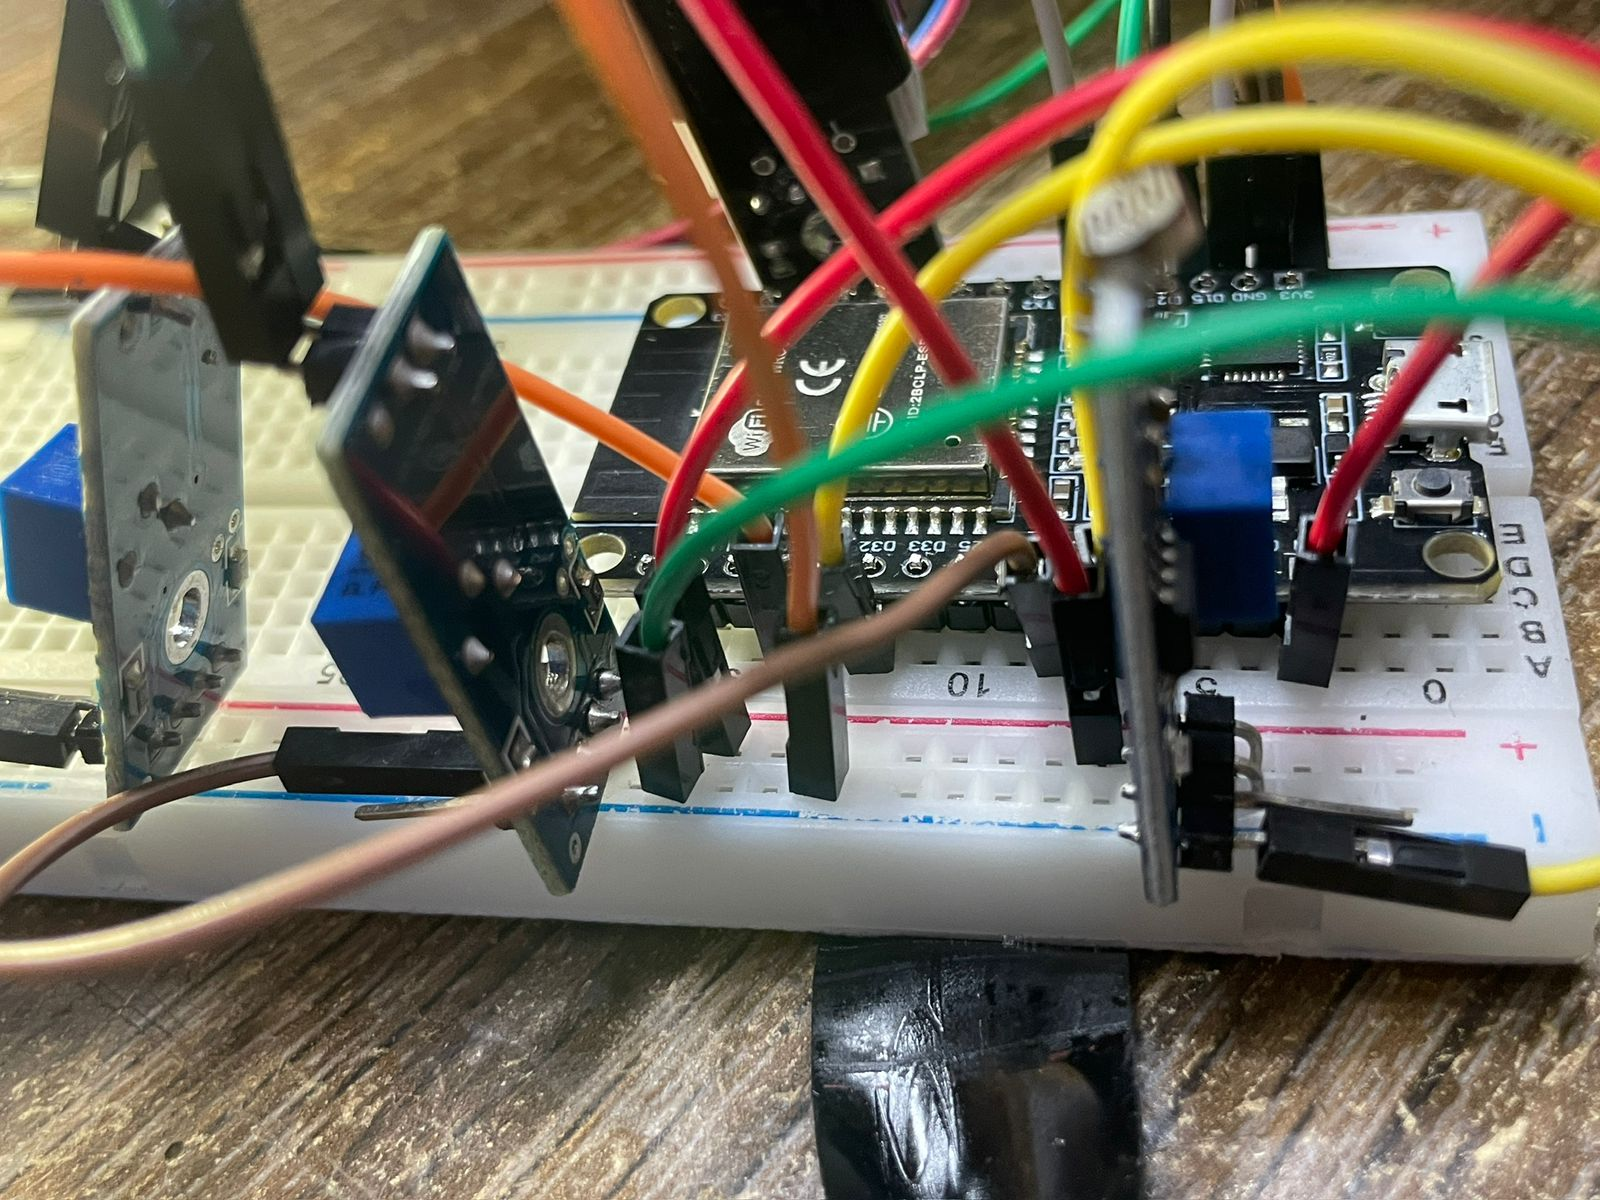
\includegraphics[width=0.85\textwidth]{figures/chapter6/sensor_pump_wiring_setup.png}
    \caption{Actuator and Sensor Wiring Configuration}
    \label{fig:sensor_pump_wiring}
\end{figure}

To validate the integration between the sensing layer and the actuation layer, Figure \ref{fig:sensor_pump_wiring} presents a close-up angle of the LDR and relay module configuration. This setup confirms the physical data pathways responsible for triggering the automated irrigation system. By isolating these specific connections, the testing phase verified that the ESP32 correctly translates logical software commands into physical electrical signals capable of safely driving the external water pump. It will comprehensively detail the purpose, underlying structure, and operational significance of the diagram, chart, or screenshot. By providing this extensive textual context, the report will ensure that readers fully understand the specific components, workflows, and technical details illustrated in the figure. (This text will be manually updated by the user once the final image is inserted).

% TODO: Required Asset Name: Field Test Environment
% Asset Type: Missing Technical Visual Asset
% Status: Pending Asset Collection
\begin{figure}[H]
    \centering
    \includegraphics[width=0.8\textwidth]{figures/chapter6/field_test_environment.png}
    \caption{[Placeholder] Field Test Environment}
    \label{fig:placeholder_field_test_environment}
\end{figure}

[PLACEHOLDER EXPLANATION]: This section serves as a 4-to-5 line explanatory paragraph that will describe the visual asset presented above. It will comprehensively detail the purpose, underlying structure, and operational significance of the diagram, chart, or screenshot. By providing this extensive textual context, the report will ensure that readers fully understand the specific components, workflows, and technical details illustrated in the figure. (This text will be manually updated by the user once the final image is inserted).


\subsection{Software \& API Testing Evidence}

To validate the software components, including the Node.js backend API, the ESP32 firmware telemetry, and the AI model outputs, rigorous software testing was conducted. The following figures provide direct visual evidence of the system's operational logs, API responses, and accurate data handling mechanisms.

% TODO: Required Asset Name: Serial Monitor Logs
% Asset Type: Missing Technical Visual Asset
% Status: Pending Asset Collection
\begin{figure}[H]
    \centering
    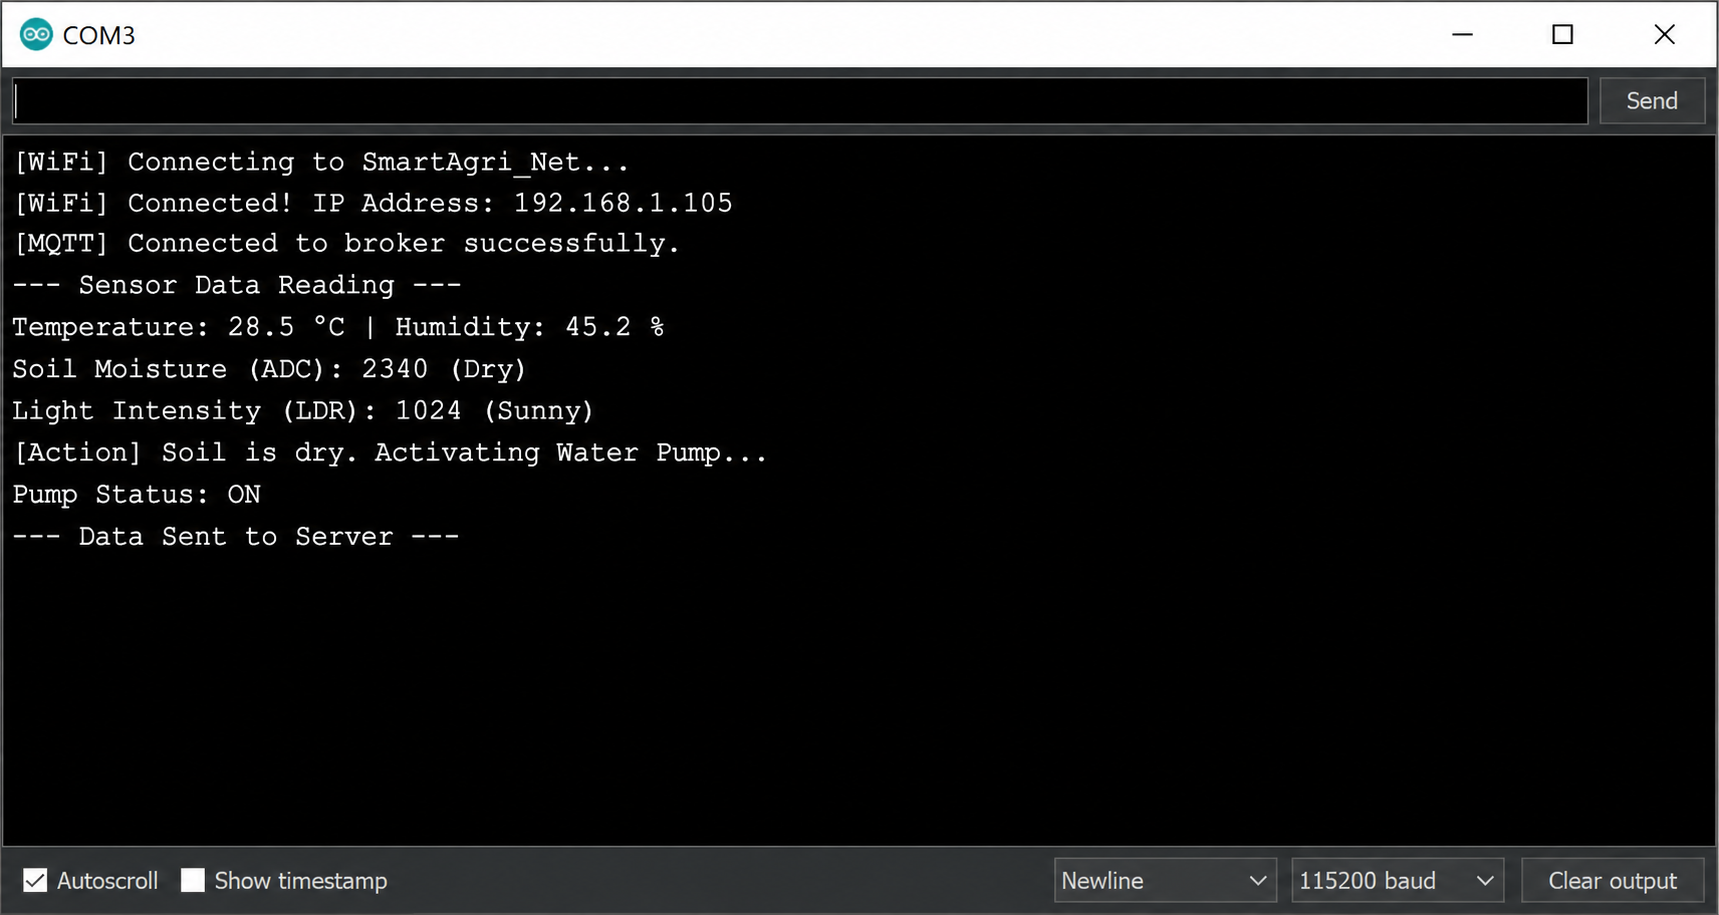
\includegraphics[width=0.8\textwidth]{figures/chapter6/serial_monitor_logs.png}
    \caption{[Placeholder] Serial Monitor Logs}
    \label{fig:placeholder_serial_monitor_logs}
\end{figure}

[PLACEHOLDER EXPLANATION]: This section serves as a 4-to-5 line explanatory paragraph that will describe the visual asset presented above. It will comprehensively detail the purpose, underlying structure, and operational significance of the diagram, chart, or screenshot. By providing this extensive textual context, the report will ensure that readers fully understand the specific components, workflows, and technical details illustrated in the figure. (This text will be manually updated by the user once the final image is inserted).

% TODO: Required Asset Name: API Output Tests
% Asset Type: Missing Technical Visual Asset
% Status: Pending Asset Collection
\begin{figure}[H]
    \centering
    \includegraphics[width=0.8\textwidth]{figures/chapter6/api_output_tests.png}
    \caption{[Placeholder] API Output Tests}
    \label{fig:placeholder_api_output_tests}
\end{figure}

[PLACEHOLDER EXPLANATION]: This section serves as a 4-to-5 line explanatory paragraph that will describe the visual asset presented above. It will comprehensively detail the purpose, underlying structure, and operational significance of the diagram, chart, or screenshot. By providing this extensive textual context, the report will ensure that readers fully understand the specific components, workflows, and technical details illustrated in the figure. (This text will be manually updated by the user once the final image is inserted).

% TODO: Required Asset Name: Sensor Reading Validation
% Asset Type: Missing Technical Visual Asset
% Status: Pending Asset Collection
\begin{figure}[H]
    \centering
    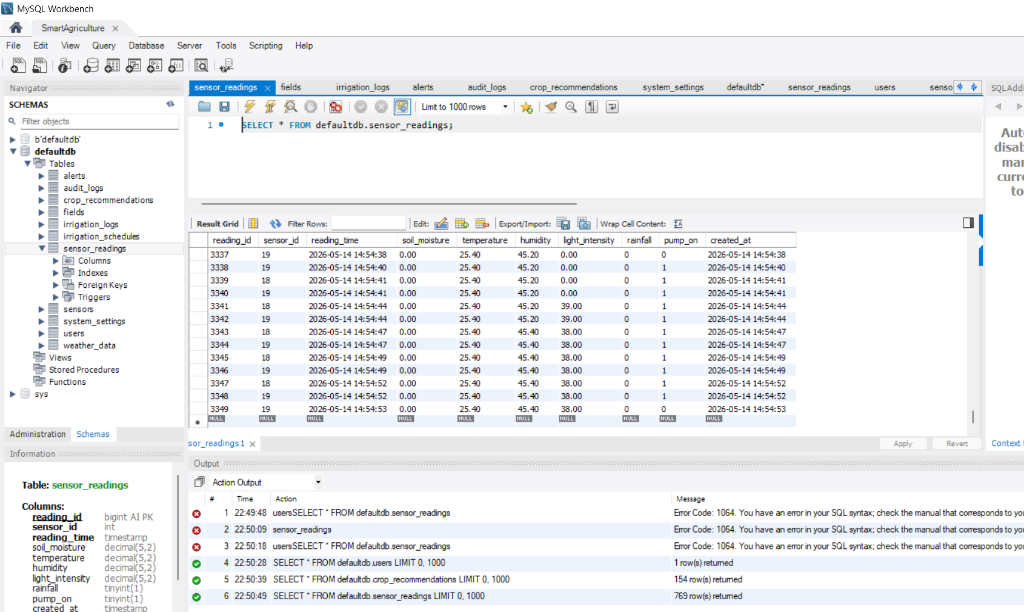
\includegraphics[width=0.8\textwidth]{figures/chapter6/sensor_reading_validation.png}
    \caption{[Placeholder] Sensor Reading Validation}
    \label{fig:placeholder_sensor_reading_validation}
\end{figure}

[PLACEHOLDER EXPLANATION]: This section serves as a 4-to-5 line explanatory paragraph that will describe the visual asset presented above. It will comprehensively detail the purpose, underlying structure, and operational significance of the diagram, chart, or screenshot. By providing this extensive textual context, the report will ensure that readers fully understand the specific components, workflows, and technical details illustrated in the figure. (This text will be manually updated by the user once the final image is inserted).

\subsection{Summary}

A total of \textbf{31 test cases} were designed and
executed across four levels of testing: 10 Unit Tests,
7 Component Tests, 7 Integration Tests, and 10 System
Tests. All 31 test cases passed successfully, confirming
that the Smart AI Powered Agriculture System meets all
functional requirements defined in Chapter~2
\cite{tahir2019traceability}. The testing process
validated every major system module including sensor
firmware, automated and manual irrigation control,
push notifications, AI crop recommendations, historical
analytics, data export, field comparison, sensor offline
detection, and network failure resilience
\cite{jaliyagoda2023iot, sommerville2016software}.
The complete test results demonstrate a fully functional,
integrated, and reliable end-to-end smart agriculture
platform.

\setcounter{chapter}{6}